%% =====================================================================
%%  Benchmarking General and Medical Small Language Models for
%%  Spanish Obstetric Question Answering: The Impact of Fine-Tuning
%%
%%  IEEE conference template (IEEEtran.cls).
%%  Build: pdflatex -> bibtex -> pdflatex -> pdflatex
%%
%%  Class options:
%%    conference : IEEE conference/symposium style (two columns, full-width
%%                 title block, "Abstract" run-in head, "Index Terms").
%%    Use [journal] instead for IEEE Transactions/Journals submission.
%%
%%  Deliberately NOT loaded (incompatible with IEEEtran or forbidden by
%%  the IEEE template): geometry, caption, float, placeins, newtxtext,
%%  newtxmath, inputenc, enumitem, dblfloatfix, stfloats, xcolor.
%%
%%  stfloats is omitted on purpose: the IEEEtran HOWTO documents it as a
%%  "very invasive package" needed only for double-column floats at the
%%  BOTTOM of a page (\begin{figure*}[!b]). Every full-width float here is
%%  placed at the top, so it would add output-routine risk with no benefit.
%% =====================================================================
\documentclass[conference]{IEEEtran}

% --- Fonts and encoding ---------------------------------------------
\usepackage[T1]{fontenc}

% --- Mathematics ----------------------------------------------------
\usepackage{amsmath,amssymb,amsfonts}

% --- Graphics, floats and tables ------------------------------------
\usepackage{graphicx}
% needspace keeps a short paragraph from being split by a full-width float:
% it breaks the column instead of letting the text straddle the float.
\usepackage{needspace}
\usepackage{booktabs}          % \toprule \midrule \bottomrule \cmidrule

\usepackage{array}
\usepackage[caption=false]{subfig}  % sub-figures; caption=false is required
                                    % because the caption package must not be
                                    % used together with IEEEtran
\usepackage{threeparttable}    % professional table notes
\usepackage{textcomp}

% Avoid stacking full-width tables on one page or multiple figures in one
% column, keeping the float sequence close to the relevant explanations.
\setcounter{topnumber}{1}
\setcounter{dbltopnumber}{1}

% --- Citations and hyperlinks ---------------------------------------
\usepackage{cite}              % IEEE-recommended numeric citation handling

% --- Typographic fine-tuning ----------------------------------------
% microtype is loaded before hyperref so that both patch the output routine
% and the PDF-string machinery in the documented order.
\usepackage{microtype}

\usepackage[hidelinks]{hyperref}

% --- Project-local shorthands ---------------------------------------
% \code marks technical identifiers (model ids, paths, configuration keys).
% It is declared as a URL-style command instead of plain \texttt so that a
% long monospaced token may break instead of overflowing its column.
% Two consequences to keep in mind:
%   * the argument is read verbatim, so write the underscore directly;
%   * it is URL-like, so spaces inside the argument are NOT preserved. Use it
%     for single tokens only.
% \UrlBreaks below is url's default break list with two edits: the underscore
% is removed (breaking an identifier at "_" reads as two separate words,
% e.g. "clinical_" / "score") and the hyphen is added (url does not break on
% hyphens by default, which matters for long model ids).
\def\UrlBreaks{\do\.\do\@\do\\\do\/\do\!\do\|\do\;\do\>\do\]%
  \do\)\do\,\do\?\do\'\do+\do\=\do\#\do\-}
\DeclareUrlCommand\code{\urlstyle{tt}}
\newcommand{\dash}{---}

\begin{document}

% =====================================================================
%  Title, authors and affiliations
%  IEEE rule: title in upper and lower case, never all upper case, and no
%  symbols, math, footnotes or citations inside the title.
%
%  Author block: each author gets its own \IEEEauthorblockN plus one
%  \IEEEauthorblockA, separated by \and. IEEEtran lays these out in columns,
%  matching the official IEEE conference template (name, then dept./org. in
%  italic, then City, Country upright, then email address or ORCID).
% =====================================================================
\title{Benchmarking General and Medical Small Language Models for
Spanish Obstetric Question Answering: The Impact of Fine-Tuning}

\author{%
\IEEEauthorblockN{Jhon H. Mej\'ia-Muñoz}
\IEEEauthorblockA{\textit{Facultad de Ingenier\'ia, IUE}\\
Envigado, Colombia\\
ORCID: 0009-0008-7768-4072}
\and
\IEEEauthorblockN{Nicol\'as Hoyos-Giraldo}
\IEEEauthorblockA{\textit{Facultad de Ingenier\'ia, IUE}\\
Envigado, Colombia\\
ORCID: 0009-0008-7768-4072}
\and
\IEEEauthorblockN{Daniel Betancur-Vasquez}
\IEEEauthorblockA{\textit{Facultad de Ingenier\'ia, IUE}\\
Envigado, Colombia}
\and
\IEEEauthorblockN{Kevin D. Trujillo}
\IEEEauthorblockA{\textit{Facultad de Ingenier\'ia, IUE}\\
Envigado, Colombia}
}

\maketitle

% =====================================================================
%  Abstract and index terms
%  IEEE order: \maketitle, then abstract, then IEEEkeywords.
% =====================================================================
\begin{abstract}
Small Language Models (SLMs) offer a computationally efficient alternative
to large language models for clinical question answering; however, evidence
on domain adaptation for Spanish obstetric applications remains limited.
This study compares the general-purpose Gemma~4 model and the medically
pretrained MedGemma~1.5 before and after grounded QLoRA adaptation using
MaternaQA-es, while examining No RAG, Hybrid retrieval, and
independent HyDE as experimental factors. All 24 scenario-condition runs
were evaluated across two 10-question scenarios, yielding 240 final
condition-item outputs. Within this exploratory evaluation, Gemma~4 Base
with Hybrid retrieval achieved the highest observed Answer Correctness and
Semantic Similarity in both scenarios, whereas MedGemma~1.5 QLoRA with
No RAG achieved the highest observed mean Answer Relevancy. HyDE
generally improved retrieval precision relative to Hybrid, especially in
the obstetric challenge scenario, but its effects on answer quality were
heterogeneous and model-dependent. Under No RAG, QLoRA improved all three
response metrics for Gemma~4 in both scenarios and for MedGemma~1.5 in the
obstetric challenge set, while the MaternaQA-es subset showed a
correctness-relevance trade-off for MedGemma~1.5. Given the limited
evaluation of 10 questions per scenario, these findings should be
interpreted as preliminary descriptive patterns rather than definitive
evidence of model or retrieval-strategy superiority. Broader evaluation and
clinician review are needed.
\end{abstract}

\begin{IEEEkeywords}
Small language models, QLoRA, retrieval-augmented generation, HyDE,
obstetric question answering, Spanish clinical NLP, model benchmarking.
\end{IEEEkeywords}

% =====================================================================
\section{Introduction}
% =====================================================================
The rapid adoption of Large Language Models (LLMs) has transformed the
development of clinical decision-support systems and medical
question-answering (QA) applications. Nevertheless, their computational
requirements limit deployment in many healthcare environments, motivating
increasing interest in Small Language Models (SLMs), which offer lower
inference costs, reduced hardware requirements, and easier local
deployment while maintaining competitive performance in domain-specific
tasks~\cite{pingua2025medical,gemma2024}. In medical applications,
supervised fine-tuning has emerged as a practical strategy for adapting
compact language models to specialized clinical domains while preserving
computational efficiency.

Recent studies have shown that domain-specific fine-tuning and retrieval
can improve medical question answering under resource
constraints~\cite{bora2024systematic}. Work on fine-tuned clinical
embedding models likewise demonstrates the value of domain-specific
retrieval, but remains outside Spanish obstetric QA~\cite{arzideh2026improving}.
Recent obstetric applications include simulated-case decision support,
emergency-response evaluation, and neonatal growth
prediction~\cite{psilopatis2026role,arslan2025evaluation,xu2026obstet}.
Reviews of maternal-health RAG emphasize the lack of standardized
benchmarks and clinically validated evaluation
protocols~\cite{noguera2025applications}. This gap is especially relevant
in obstetric care, where inaccurate recommendations may affect maternal
and fetal safety~\cite{pacheco2023inteligencia}.

An important question therefore remains: does medical pretraining continue
to provide measurable advantages after domain-specific fine-tuning?
Medically pretrained SLMs should encode biomedical terminology, clinical
concepts, and reasoning patterns. Yet, after both a general-purpose and a
medical model receive identical specialized supervision, it remains unclear
whether prior medical knowledge provides an additional benefit or whether
the general-purpose model can achieve comparable or superior performance.

To investigate this question, this study uses MaternaQA-es, a Spanish
obstetric QA resource containing 5,727 synthetic question-answer pairs
generated from 63 Spanish-language clinical documents. The dataset is
publicly available through
Hugging Face~\cite{maternaqa2026}. The benchmark compares Gemma~4 and
MedGemma~1.5 before and after identical grounded QLoRA adaptation.

This work makes three contributions. First, it compares general-purpose and
medically pretrained SLMs for Spanish obstetric QA. Second, it evaluates
the effect of domain-specific QLoRA adaptation under matched training
conditions. Third, it provides a reproducible experimental design that
incorporates retrieval-augmented inference and item-level evaluation while
explicitly separating completed runs from planned factorial conditions.

% =====================================================================
\section{Methodology}
% =====================================================================
\subsection{Study Design and Research Questions}
The study uses a controlled, offline factorial benchmark. Model family has
two levels: Google Gemma~4 E2B instruction-tuned
(\code{google/gemma-4-E2B-it}) and Google MedGemma~1.5 4B instruction-tuned
(\code{google/medgemma-1.5-4b-it}). Parameter adaptation has two levels:
base weights without an adapter and grounded QLoRA. Retrieval strategy has
three planned levels: the No RAG control, canonical
Hybrid retrieval, and canonical independent HyDE. Their Cartesian product
defines 12 planned conditions.

The unit of analysis is an item-level paired \code{qa_id}. The primary
QLoRA estimand is the paired difference between QLoRA and base outputs
within a fixed model family and retrieval strategy. Retrieval contrasts
compare strategies within a fixed family and adaptation state. The
interaction estimand is the change in the QLoRA effect across retrieval
strategies:
\begin{equation}
\label{eq:interaction}
\Delta = (Y_{Q,H} - Y_{B,H}) - (Y_{Q,N} - Y_{B,N}).
\end{equation}
Here $Q$ denotes QLoRA, $B$ denotes the base model, $H$ denotes Hybrid
retrieval, and $N$ denotes the No RAG condition. Analogous contrasts
are defined for HyDE and for the two model families.

\subsection{Dataset, Provenance, and Split Integrity}
MaternaQA-es contains 5,727 Spanish obstetric question-answer pairs derived
from 63 clinical documents. Its document-level partitions contain 52
training PDFs (5,093 items), 2 validation PDFs (306 items), and 3 held-out
test PDFs. This study processed 10 test questions; test
sources do not overlap training or validation sources, and \code{qa_id} is
retained as the pairing key~\cite{maternaqa2026}.

The primary grounded adaptation uses the \code{sft_grounded}
representation, in which the source context associated with an item is
concatenated with the question. The term base indicates whether an adapter is
loaded; it does not indicate that the input is closed-book when context is
otherwise present.

The same 10 held-out test questions were processed across all model and
retrieval conditions. The 2,268-chunk retrieval corpus includes the source
material associated with these questions. Therefore, the RAG evaluation
measures the system's ability to retrieve and use relevant evidence when
that evidence is available in the corpus, rather than strict generalization
to completely unseen source documents. This inference-time access is
distinct from leakage into model parameters, because the corresponding test
documents were not used during fine-tuning.

\subsection{Protocol Evaluation Scenarios}
Two protocol scenarios define the evaluation inputs. The first is a
10-item obstetric challenge set represented by \code{datasets/sample10.jsonl};
these records do not provide document-level reference chunk identifiers.
The second consists of 10 processed questions from the held-out MaternaQA-es
test partition, with QA metadata and source-reference information.
MaternaQA-es is publicly available on Hugging Face~\cite{maternaqa2026}.

The challenge set supports answer-quality evaluation but not gold
document-level retrieval recall. The processed MaternaQA-es subset supports
both response metrics and reference-chunk checks. Each scenario used 10
questions across all 12 conditions. MaternaQA-es preserves grounded source
context with the question, whereas \code{sample10} contains only the
question before retrieval-stage context is added. This input difference may
affect the results.

Therefore, the two scenarios are treated as complementary evaluation
settings rather than directly comparable samples from the same input
distribution. Absolute metric differences between MaternaQA-es and the
obstetric challenge set are not interpreted as effects of fine-tuning or
retrieval, because scenario membership is confounded with differences in
input construction and source-context availability. Model and retrieval
comparisons are consequently emphasized within each scenario.

\subsection{Model Families and Experimental Conditions}
The benchmark compares Google Gemma~4 E2B instruction-tuned with Google
MedGemma~1.5 4B instruction-tuned. Base conditions load the published
model without an adapter. QLoRA conditions load
\code{iue-edu/MaternaCare-ES-gemma4-qlora} or
\code{iue-edu/MaternaCare-ES-medgemma-qlora} on the corresponding base
model. The answer model, decoding settings, prompt structure, and test
items are held fixed across retrieval strategies within a family and
adaptation state.

Table~\ref{tab:factorial} lists the complete prespecified design. The final
result artifacts covered No RAG, Hybrid, and HyDE for all four
model/adaptation combinations in both scenarios; therefore, all 24
scenario-condition runs were represented in the analysis.

% --- Table I: full-width, caption above, no vertical rules -----------
\begin{table*}[t]
\centering
\begin{threeparttable}
\caption{Prespecified Factorial Experiment Matrix}
\label{tab:factorial}
\scriptsize
\begin{tabular*}{\textwidth}{@{\extracolsep{\fill}}c l l l p{0.40\textwidth}@{}}
\toprule
ID & Model family & Adaptation & Retrieval & Condition definition \\
\midrule
C01 & Gemma 4 & Base & No RAG & Base weights; no retrieved context \\
C02 & Gemma 4 & Base & Hybrid & Base weights; canonical Hybrid retrieval \\
C03 & Gemma 4 & Base & HyDE & Base weights; canonical independent HyDE retrieval \\
C04 & Gemma 4 & QLoRA & No RAG & Grounded QLoRA adapter; no retrieved context \\
C05 & Gemma 4 & QLoRA & Hybrid & Grounded QLoRA adapter; canonical Hybrid retrieval \\
C06 & Gemma 4 & QLoRA & HyDE & Grounded QLoRA adapter; canonical independent HyDE retrieval \\
C07 & MedGemma 1.5 & Base & No RAG & Base weights; no retrieved context \\
C08 & MedGemma 1.5 & Base & Hybrid & Base weights; canonical Hybrid retrieval \\
C09 & MedGemma 1.5 & Base & HyDE & Base weights; canonical independent HyDE retrieval \\
C10 & MedGemma 1.5 & QLoRA & No RAG & Grounded QLoRA adapter; no retrieved context \\
C11 & MedGemma 1.5 & QLoRA & Hybrid & Grounded QLoRA adapter; canonical Hybrid retrieval \\
C12 & MedGemma 1.5 & QLoRA & HyDE & Grounded QLoRA adapter; canonical independent HyDE retrieval \\
\bottomrule
\end{tabular*}
\begin{tablenotes}[flushleft]
\item[] \textit{Note.} The complete design is 2 model families $\times$
2 adaptation states $\times$ 3 retrieval strategies. All 12 conditions were
observed in each of the two evaluation scenarios.
\end{tablenotes}
\end{threeparttable}
\end{table*}

\subsection{Grounded QLoRA Fine-Tuning}
QLoRA~\cite{dettmers2023qlora} is the parameter-adaptation method in the
benchmark: trainable low-rank adapters on quantized base weights, which
keeps the base model as a separately identifiable initialization.
Fig.~\ref{fig:qlora} contrasts it with full fine-tuning, and
Table~\ref{tab:qlora-config} specifies the NF4 quantization and BF16
computation settings.

% The paragraph below must not straddle the Table I float on the next page:
% without this it ends on "...both models. Table II" and the reader finds the
% verb after a full-width table, which also misreads as if it referred to Table I.
\needspace{8\baselineskip}
Both model families used the same MaternaQA-es training and validation
partitions and the same grounded input representation. To maintain a
controlled comparison between model initializations, the QLoRA
hyperparameters and optimization settings were held constant across both
models. Table~\ref{tab:qlora-config} summarizes the training configuration
used to produce the evaluated adapters.

% --- Table II: full-width, caption above, no vertical rules ----------
\begin{table*}[t]
\centering
\begin{threeparttable}
\caption{QLoRA Fine-Tuning Configuration Used for Both Model Families}
\label{tab:qlora-config}
\scriptsize
% tabular* + \extracolsep{\fill} spans exactly \textwidth: the model
% identifiers do not fit a single column, so the float is table* and the
% columns are spread deliberately instead of being hand-padded.
\begin{tabular*}{\textwidth}{@{\extracolsep{\fill}}lcc@{}}
\toprule
Parameter & Gemma 4 E2B QLoRA & MedGemma 1.5 4B QLoRA \\
\midrule
Base model & google/gemma-4-E2B-it & google/medgemma-1.5-4b-it \\
Training representation & sft\_grounded & sft\_grounded \\
Train / validation examples & 5,093 / 306 & 5,093 / 306 \\
Quantization & 4-bit NF4, double quantization & 4-bit NF4, double quantization \\
LoRA rank ($r$) & 16 & 16 \\
LoRA alpha & 16 & 16 \\
LoRA dropout & 0.05 & 0.05 \\
Target modules & All linear (all-linear) & All linear (all-linear) \\
Learning rate & $2 \times 10^{-4}$ & $2 \times 10^{-4}$ \\
Batch size & 1 per device & 1 per device \\
Gradient accumulation steps & 8 & 8 \\
Effective batch size & 8 & 8 \\
Epochs / training steps & 2 / 1,274 & 2 / 1,274 \\
Optimizer & AdamW 8-bit & AdamW 8-bit \\
LR scheduler & Cosine & Cosine \\
Maximum sequence length & 1,024 & 1,024 \\
Packing & Disabled & Disabled \\
Random seed & 3407 & 3407 \\
\bottomrule
\end{tabular*}
\begin{tablenotes}[flushleft]
\item[] \textit{Note.} Both model families used the same training and
validation partitions, grounded input representation, and QLoRA
optimization settings.
\end{tablenotes}
\end{threeparttable}
\end{table*}

The \code{sft_grounded} examples use the dataset's conversational
\code{Contextofuente} representation, in which source context is presented
with the question. This differs from retrieval at inference: training
context is pre-associated with each example, whereas RAG selects contexts
from the 2,268-chunk corpus for each question. The adapter is loaded only in
QLoRA conditions.

% --- Figure 1: single-column QLoRA comparison ------------------------
\begin{figure}[t]
\centering
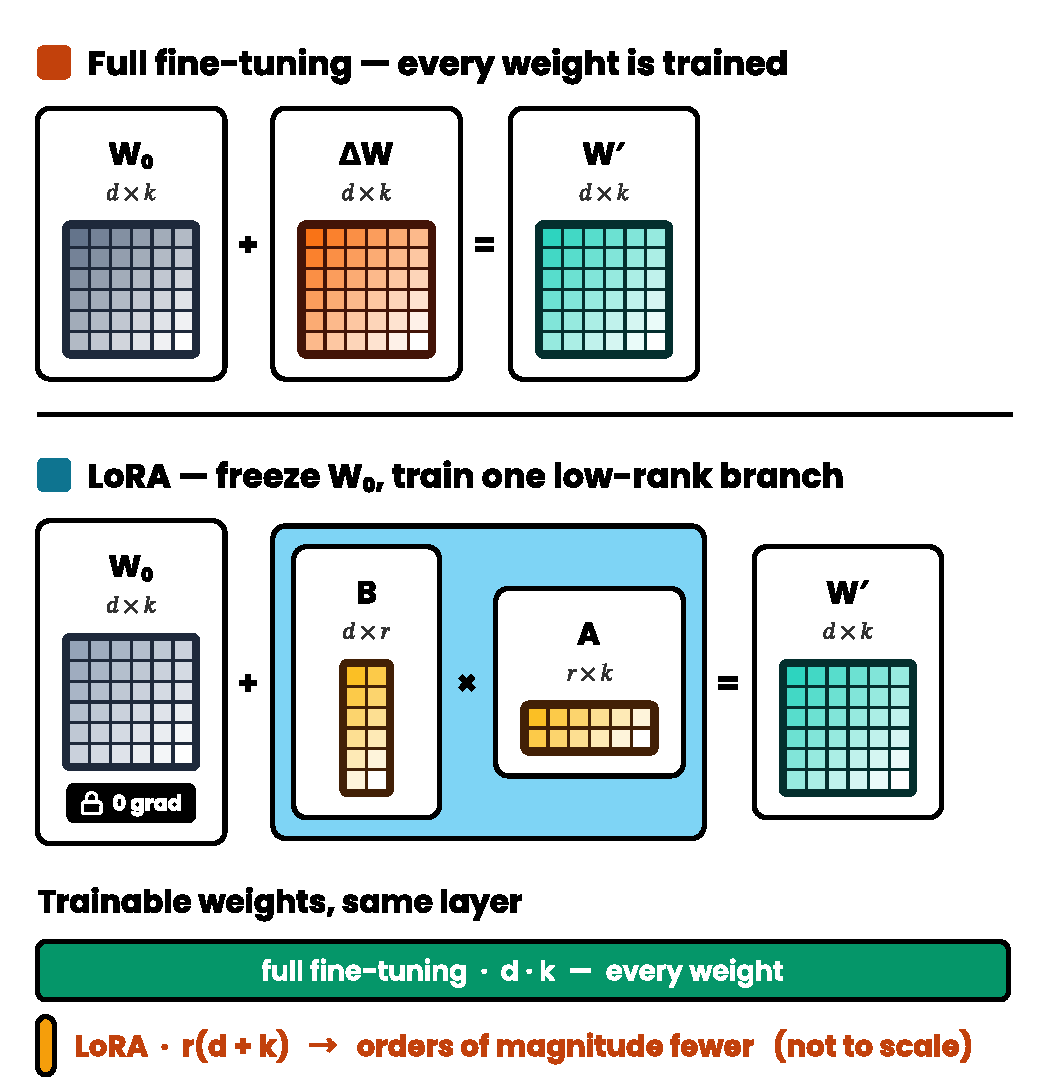
\includegraphics[width=\columnwidth]{figures/ft-vs-lora.pdf}
\caption{Comparison of full fine-tuning and LoRA adaptation.}
\label{fig:qlora}
\end{figure}

\subsection{Retrieval-Augmented Generation Protocol}
RAG is the second core method~\cite{lewis2020retrieval}. The protocol treats
retrieval strategy as a reproducible experimental factor. No RAG, Hybrid
retrieval, and independent HyDE differ in how evidence is
prepared before the answer model receives the question and context.
Hypothetical text is used only for query expansion. Fig.~\ref{fig:rag-types}
summarizes the three variants.

% --- Single-column RAG variants figure, caption below ----------------
\begin{figure}[t]
\centering
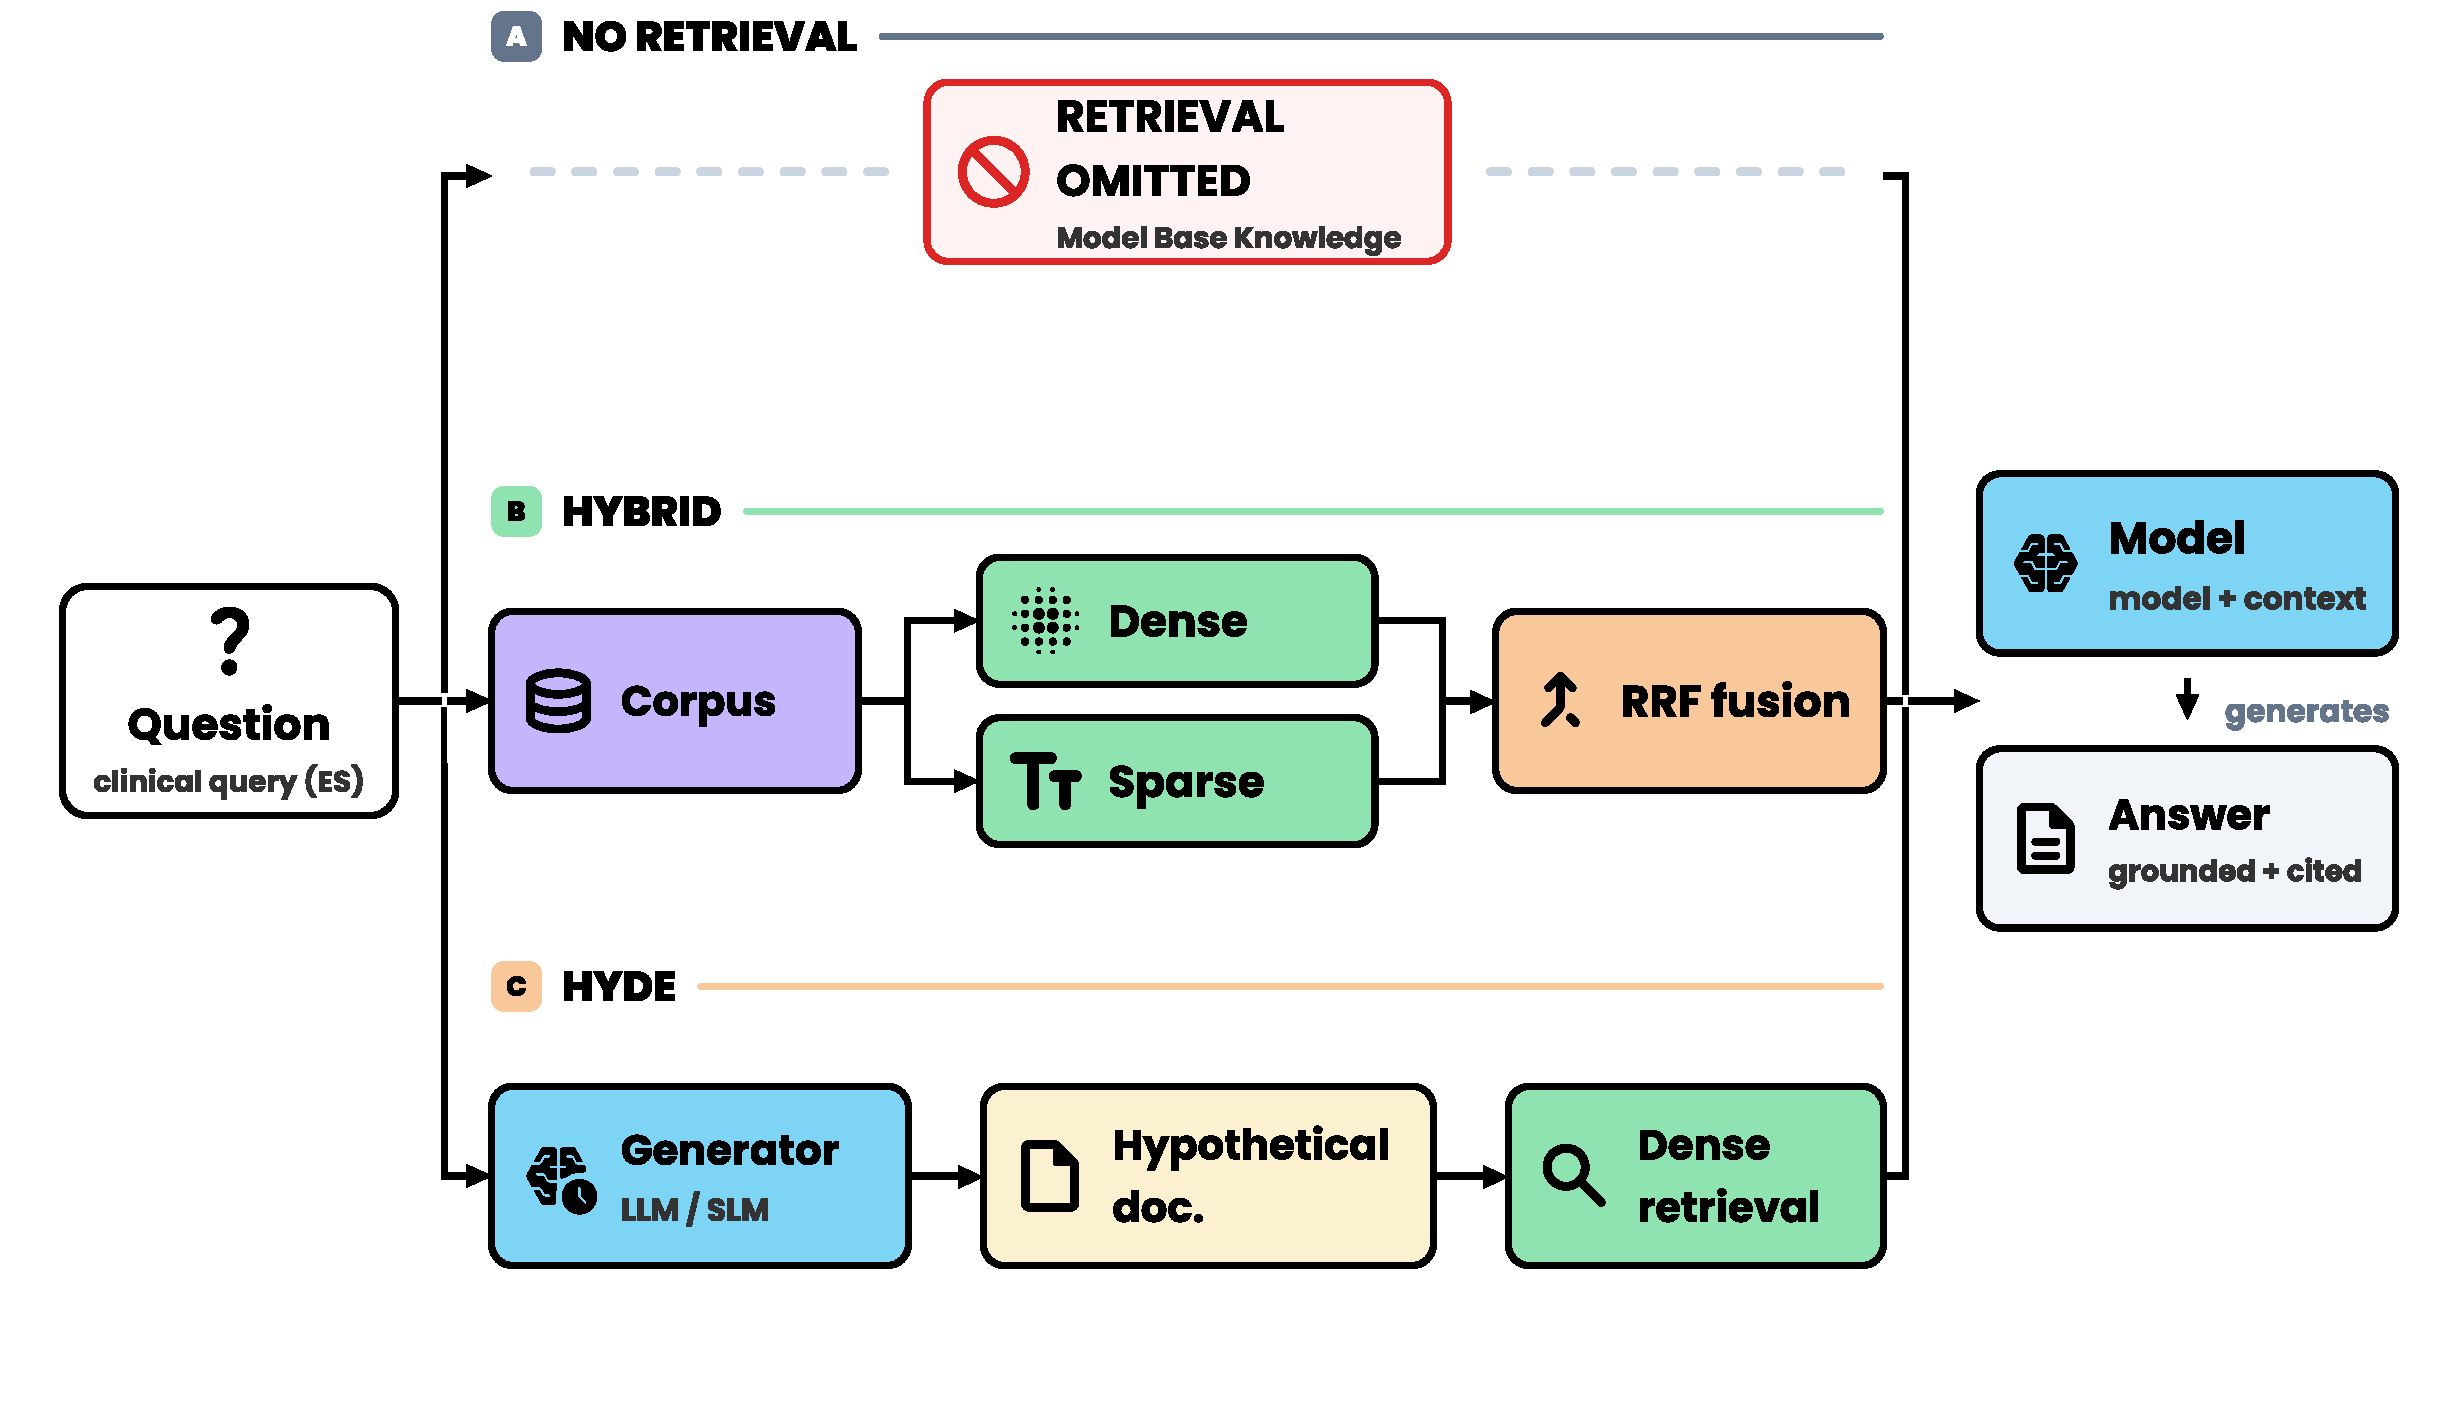
\includegraphics[width=\columnwidth]{figures/rag-types.pdf}
\caption{RAG variants used in the benchmark: No RAG, Hybrid retrieval
with dense and sparse fusion, and independent HyDE retrieval.}
\label{fig:rag-types}
\end{figure}

\subsubsection{Corpus Provenance and Chunk Construction}
The separate retrieval corpus contains 2,268 chunks from curated
obstetric source documents and is used for dense, sparse, and fused
retrieval. The \code{clinical_score} is a corpus-filtering signal, not
clinical validation.

% A single equation number for the whole scoring definition: \notag removes
% the numbers of the continuation rows, which are never referenced.
\begin{align}
S(x) &= \max\bigl\{0,\, L(x) + A(x) + B(W) - P(R)\bigr\},\\
L(x) &= \sum_{t \in T,\; t \subseteq \operatorname{norm}(x)}
        \bigl[1 + \mathbf{1}(t \text{ contains a space})\bigr],\notag\\
A(x) &= \sum_{a \in A,\; a \subseteq \operatorname{norm}(x)} 1,\notag\\
B(W) &= 2\mathbf{1}(W \geq 120) + 2\mathbf{1}(W \geq 350),\notag\\
P(R) &= 3\mathbf{1}(R \geq 0.35).\notag
\end{align}
Here $\operatorname{norm}(x)$ applies Unicode normalization, removes
combining marks, lowercases text, replaces non-ASCII letters and
punctuation with spaces, and collapses whitespace. $T$ is the
clinical-term set, $A$ the action-term set, $W$ the Unicode word count, and
$R$ the ratio of reference-matching nonempty lines to all nonempty lines.

\subsubsection{Dense and Sparse Retrieval}
Dense retrieval uses \code{BAAI/bge-m3}~\cite{chen2024bge}.
SentenceTransformer produces normalized dense vectors on CPU with
\code{batch_size=32}. The persistent local vector table is
LanceDB~\cite{lancedb2026vector}.
Because no approximate vector index is created, search is exhaustive exact
cosine search. The default dense retrieval depth is $k = 5$.

Sparse retrieval is Okapi BM25 (\code{rank_bm25/BM25Okapi}) over Unicode
lowercase word tokens. Retrieval outputs are recorded before answer
generation so retrieval quality and latency can be analyzed separately from
response generation.

\subsubsection{Canonical Hybrid Retrieval}
Hybrid retrieval fuses dense and BM25 rankings by reciprocal rank fusion
with \code{rank_constant=60}~\cite{cormack2009reciprocal}. For a requested
final depth $k$, the candidate depth is:
\begin{equation}
\label{eq:candidate-depth}
k_c = \min(\lvert C \rvert,\, \max(4k, 50)).
\end{equation}
Ties are broken by stable chunk ID, and the final top-$k$ chunks are
supplied to the answer model.

\subsubsection{Canonical Independent HyDE Retrieval}
HyDE~\cite{gao2023precise} uses a dedicated hypothetical-document
generator, separate from the answer model, to produce a Spanish
clinical-document passage from the question. The retained runs used the
OpenAI provider with \code{gpt-5-mini-2025-08-07}. Hypothetical documents
were generated once per question and cached for reuse across answer-model
conditions; dense retrieval then embeds that text with BGE-M3 and searches
the corpus by exact cosine similarity. Only the retrieved corpus chunks,
not the hypothetical text, are supplied as evidence to the answer
model~\cite{ji2023survey}. The cache is separated by dataset mode, provider,
and generator model, and row reuse checks \code{qa_id} and a question hash.

\subsubsection{No RAG Control}
The No RAG control returns no retrieved contexts and
omits the retrieved-context block from the answer prompt. Context-dependent
retrieval metrics are therefore not defined and are not assigned a value of
zero.

\subsection{Inference and Prompt Controls}
All answer prompts are written in Spanish. RAG prompts contain a clearly
delimited context block with positional labels and the question. Provenance
is retained in benchmark records rather than asserted as content in the
answer prompt. The No RAG condition receives the same question
formatting and chat template but an empty context block.

Inference uses the model's chat template and greedy decoding by default,
with a maximum of 512 newly generated tokens. Sampling is disabled unless a
run explicitly records a different configuration. QLoRA conditions load the
declared adapter on the corresponding base model; base conditions do not.
Retrieval generation and answer generation remain separate stages.

\subsection{Evaluation Framework and Metrics}
RAGAS 0.4.3~\cite{es2024ragas} is used as an external automatic evaluation
layer. It is neither the retriever nor a clinical expert.
Response-quality, retrieval-quality, and operational measurement domains
are kept separate before paired contrasts and interaction analysis.
Figure~\ref{fig:ragas-eval-workflow} illustrates the RAGAS evaluation
workflow, showing how each part contributes to scoring the responses.
\begin{figure}[!t]
\centering
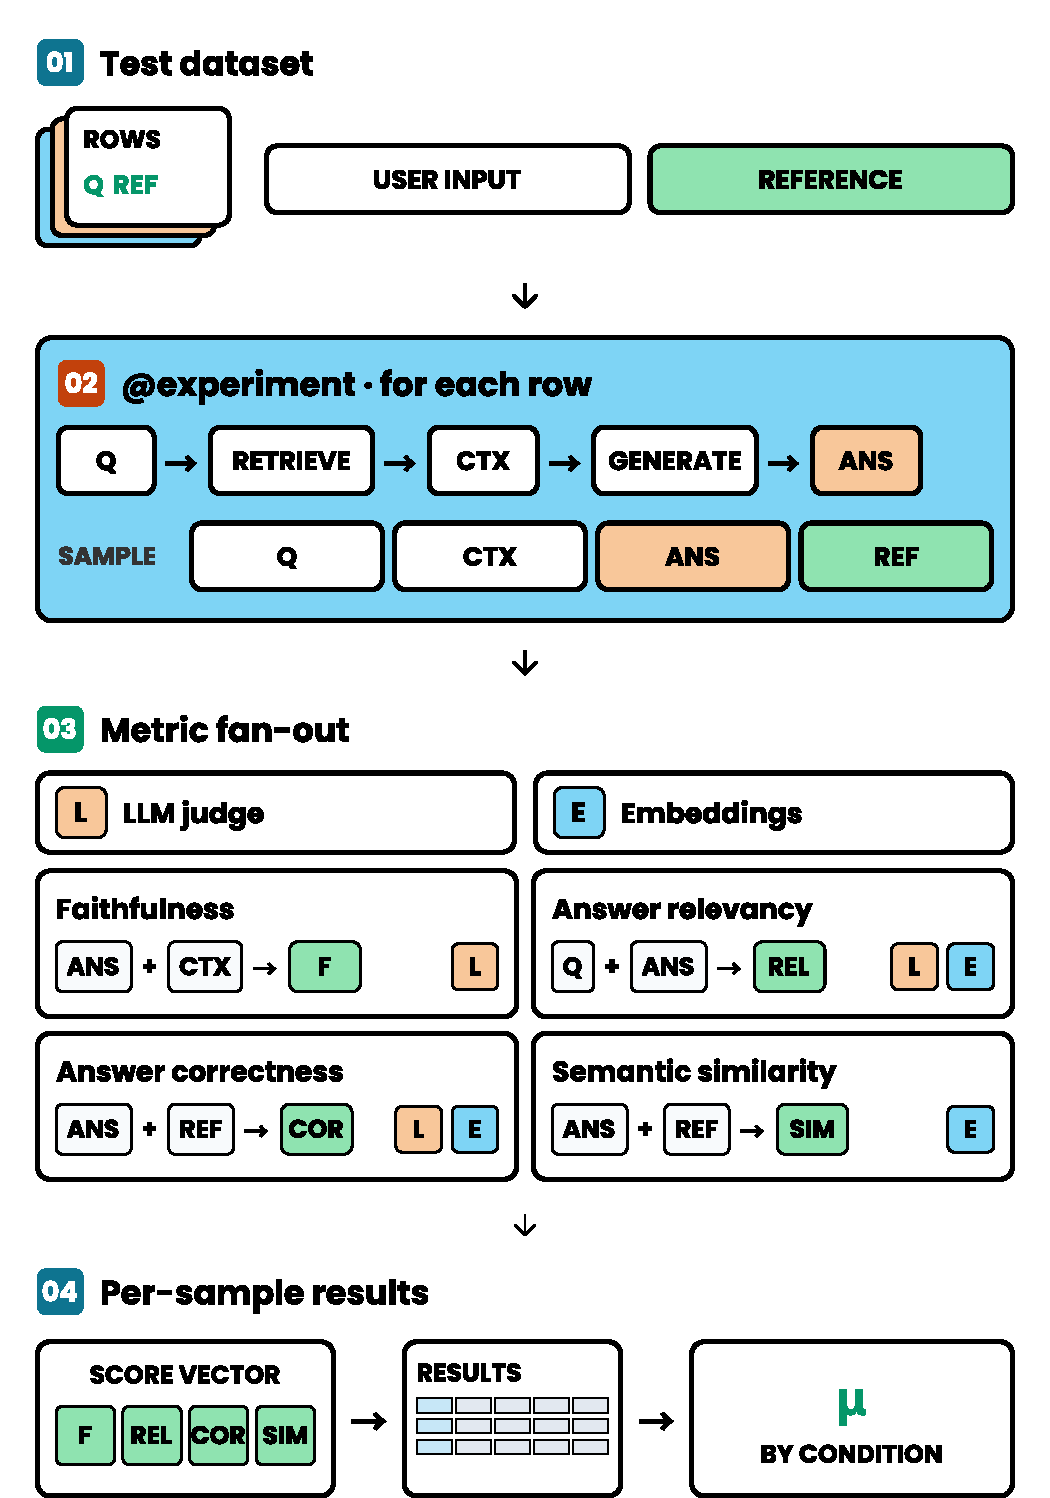
\includegraphics[width=\columnwidth]{figures/ragas-eval-workflow.pdf}
\caption{RAGAS response-evaluation workflow from per-question inputs and
evidence to per-condition results.}
\label{fig:ragas-eval-workflow}
\end{figure}

\subsubsection{Retained Fine-Tuning-Output Evaluator}
The retained evaluator uses RAGAS 0.4.3 with \code{gpt-5.4-mini} as
evaluator, \code{text-embedding-3-small} for embedding-based evaluation,
and a maximum completion length of 2,048 tokens. The retained metrics are
Faithfulness, Answer Relevancy, Answer Correctness, and Semantic Similarity.

\subsubsection{RAG Benchmark Evaluator}
The RAG evaluator uses six metrics: Context Precision, Context Recall,
Faithfulness, Answer Relevancy, Answer Correctness, and Semantic
Similarity. Their definitions follow RAGAS and are not restated here; the
scoring pipeline is summarized in Fig.~\ref{fig:ragas-eval-workflow}.

Operational variables include input, output, and total token counts;
retrieval, generation, and end-to-end latency; and output tokens per
second. Wall-clock output rate is descriptive and not treated as
hardware-independent throughput.
\begin{equation}
\label{eq:tps}
\mathrm{TPS} = \frac{N_{\mathrm{out}}}{T_{\mathrm{gen}}}.
\end{equation}

\subsection{Analysis Plan}
The primary analysis is descriptive and item-level. Means are computed from
the valid automatic scores available within each balanced 10-question
scenario. Given the limited
number of evaluated questions per scenario, all comparisons are treated as
exploratory rather than confirmatory. QLoRA is compared with
base within each retrieval strategy and family; retrieval strategies are
contrasted within adaptation and family; and model families are compared
under matched conditions.

Duplicate or superseded records were resolved at \code{qa_id} level by
preferring more complete rows, fewer metric errors, and then the latest row
position. The summary used the same 10 \code{qa_id} values shared by all 12
conditions in each scenario.

\subsection{Reproducibility and Experimental Scope}
Reproducibility requires recording the MaternaQA-es revision,
retrieval-corpus hash, complete configuration, prompts, model and adapter
identifiers, HyDE provider settings, cache identity, evaluator version, and
decoding settings. The pinned BGE-M3 revision and deterministic RRF
tie-breaking are part of this record. Reporting follows the transparency
goals of TRIPOD-LLM and Data Statements for
NLP~\cite{gallifant2025tripod,bender2018data}.

QLoRA fine-tuning and local neural-model computations were performed on an
NVIDIA GeForce RTX 5070 Ti Laptop GPU with 12~GB of dedicated VRAM.
The comparison comprised 20 questions---10 from MaternaQA-es and 10 from
\code{sample10}---evaluated across all 12 conditions, and all principal
comparisons are made within each scenario.

% =====================================================================
\section{Results}
% =====================================================================
\subsection{Available Runs and Analysis Set}
The consolidated workbook contained 262 records, including duplicate,
retried, or superseded rows, and represented two scenarios, four model
conditions, and all three inference strategies. No RAG, Hybrid, and
HyDE were available for every model/adaptation combination in both
scenarios, completing the 12-condition matrix for each scenario.

After resolving duplicate or superseded rows and restricting both scenarios
to identifiers shared by all 12 conditions, the balanced analysis contained
240 final condition-item outputs: 120 for the MaternaQA-es subset and 120
for the obstetric challenge set. Every condition contributed responses for
all 10 questions; however, 20 condition-item records contained at least one
unavailable automatic metric, so means were calculated from valid scores
without imputation.

% --- Table III: full-width, caption above, no vertical rules ---------
\begin{table*}[!t]
\centering
\begin{threeparttable}
\caption{Mean Automatic Metrics for the 10 Shared Questions in Each Scenario}
\label{tab:results}
\scriptsize
\begin{tabular*}{\textwidth}{@{\extracolsep{\fill}}lllrrrrrr@{}}
\toprule
Model & State & Strategy & Correct. & Relev. & Sem. sim. & Faith. & C. prec. & C. recall \\
\midrule
\multicolumn{9}{c}{\textit{Panel A. MaternaQA-es test subset}} \\
\midrule
Gemma 4 & Base & No RAG & 0.320 & 0.689 & 0.684 & \dash & \dash & \dash \\
Gemma 4 & Base & Hybrid & \textbf{0.668} & 0.786 & \textbf{0.813} & 0.917 & 0.945 & \textbf{0.900} \\
Gemma 4 & Base & HyDE & 0.656 & 0.710 & 0.802 & \textbf{1.000} & 0.964 & 0.850 \\
Gemma 4 & QLoRA & No RAG & 0.449 & 0.736 & 0.737 & \dash & \dash & \dash \\
Gemma 4 & QLoRA & Hybrid & 0.451 & 0.728 & 0.791 & 0.768 & \textbf{1.000} & \textbf{0.900} \\
Gemma 4 & QLoRA & HyDE & 0.387 & 0.643 & 0.699 & 0.904 & 0.933 & 0.850 \\
MedGemma 1.5 & Base & No RAG & 0.367 & 0.599 & 0.625 & \dash & \dash & \dash \\
MedGemma 1.5 & Base & Hybrid & 0.499 & 0.562 & 0.607 & 0.790 & 0.945 & 0.850 \\
MedGemma 1.5 & Base & HyDE & 0.474 & 0.697 & 0.631 & 0.869 & 0.958 & 0.850 \\
MedGemma 1.5 & QLoRA & No RAG & 0.311 & \textbf{0.811} & 0.733 & \dash & \dash & \dash \\
MedGemma 1.5 & QLoRA & Hybrid & 0.346 & 0.706 & 0.749 & 0.841 & 0.900 & 0.812 \\
MedGemma 1.5 & QLoRA & HyDE & 0.388 & 0.649 & 0.754 & 0.761 & 0.958 & \textbf{0.900} \\
\midrule
\multicolumn{9}{c}{\textit{Panel B. Obstetric challenge set}} \\
\midrule
Gemma 4 & Base & No RAG & 0.206 & 0.708 & 0.620 & \dash & \dash & \dash \\
Gemma 4 & Base & Hybrid & \textbf{0.481} & 0.692 & \textbf{0.736} & \textbf{0.986} & 0.760 & 0.550 \\
Gemma 4 & Base & HyDE & 0.423 & 0.760 & 0.722 & 0.960 & 0.917 & \textbf{0.800} \\
Gemma 4 & QLoRA & No RAG & 0.268 & 0.824 & 0.648 & \dash & \dash & \dash \\
Gemma 4 & QLoRA & Hybrid & 0.370 & 0.647 & 0.672 & 0.898 & 0.796 & 0.500 \\
Gemma 4 & QLoRA & HyDE & 0.368 & 0.676 & 0.695 & 0.894 & 0.898 & 0.600 \\
MedGemma 1.5 & Base & No RAG & 0.216 & 0.833 & 0.620 & \dash & \dash & \dash \\
MedGemma 1.5 & Base & Hybrid & 0.240 & 0.388 & 0.509 & 0.930 & 0.811 & 0.500 \\
MedGemma 1.5 & Base & HyDE & 0.368 & 0.607 & 0.535 & 0.885 & 0.908 & 0.700 \\
MedGemma 1.5 & QLoRA & No RAG & 0.274 & \textbf{0.881} & 0.652 & \dash & \dash & \dash \\
MedGemma 1.5 & QLoRA & Hybrid & 0.373 & 0.741 & 0.685 & 0.590 & 0.841 & 0.714 \\
MedGemma 1.5 & QLoRA & HyDE & 0.256 & 0.696 & 0.660 & 0.764 & \textbf{0.919} & 0.700 \\
\bottomrule
\end{tabular*}
\begin{tablenotes}[flushleft]
\item[] \textit{Note.} Correct. = answer correctness; Relev. = answer
relevancy; Sem. sim. = semantic similarity; Faith. = faithfulness;
C. prec. = context precision; C. recall = context recall. Dashes mark
non-applicability for No RAG. All conditions yielded 10 responses;
valid $n$ was 5--10 for response metrics and 6--10 for retrieval metrics;
 bold values are panel maxima.
\end{tablenotes}
\end{threeparttable}
\end{table*}

\subsection{MaternaQA-es Subset}
Gemma~4 Base with Hybrid retrieval achieved the highest observed mean Answer
Correctness (0.668) and Semantic Similarity (0.813), while MedGemma~1.5
QLoRA with No RAG obtained the highest observed mean Answer Relevancy
(0.811). Under No RAG, QLoRA increased Gemma~4 Answer Correctness by
0.129, Answer Relevancy by 0.047, and Semantic Similarity by 0.053. For
MedGemma~1.5, QLoRA reduced Answer Correctness by 0.057 but increased
Answer Relevancy by 0.212 and Semantic Similarity by 0.109.

Relative to No RAG, Hybrid and HyDE produced their largest
response-quality gains for Gemma~4 Base: Answer Correctness increased by
0.348 with Hybrid and 0.336 with HyDE. HyDE also increased Answer
Correctness for MedGemma~1.5 Base (+0.107) and QLoRA (+0.077), but reduced
it for Gemma~4 QLoRA ($-$0.062). Directly against Hybrid, HyDE improved
Answer Correctness only for MedGemma~1.5 QLoRA (+0.042) and improved Answer
Relevancy most clearly for MedGemma~1.5 Base (+0.135), illustrating
heterogeneous retrieval effects.

\subsection{Obstetric Challenge Set}
Within the evaluated obstetric challenge subset, Gemma~4 Base with Hybrid
retrieval achieved the highest observed mean Answer Correctness (0.481) and
Semantic Similarity (0.736), whereas MedGemma~1.5 QLoRA with No RAG obtained
the highest observed mean Answer Relevancy (0.881). Under No RAG, QLoRA
improved all three response metrics for both model families.

Relative to No RAG, Hybrid increased Answer Correctness for all
four model conditions but reduced Answer Relevancy in every condition.
Semantic Similarity increased for both Gemma~4 conditions and MedGemma~1.5
QLoRA, but decreased for MedGemma~1.5 Base.

Relative to No RAG, HyDE increased Answer Correctness for Gemma~4
Base (+0.218), Gemma~4 QLoRA (+0.100), and MedGemma~1.5 Base (+0.152), but
slightly reduced it for MedGemma~1.5 QLoRA ($-$0.018). Answer Relevancy
increased only for Gemma~4 Base, while Semantic Similarity increased for
both Gemma~4 conditions and MedGemma~1.5 QLoRA but decreased for
MedGemma~1.5 Base.

Compared directly with Hybrid retrieval, HyDE improved Answer Relevancy for
both Gemma~4 conditions and MedGemma~1.5 Base, and it improved Answer
Correctness most clearly for MedGemma~1.5 Base (+0.127). It did not
dominate Hybrid for the other model conditions, confirming that
hypothetical-document expansion changed retrieval quality without
guaranteeing better final answers.

\subsection{Retrieval-Grounding Metrics}
In the MaternaQA-es subset, Hybrid Context Precision ranged from 0.900 to
1.000, Context Recall from 0.813 to 0.900, and Faithfulness from 0.768 to
0.917. HyDE Context Precision ranged from 0.933 to 0.964, Context Recall
from 0.850 to 0.900, and Faithfulness from 0.761 to 1.000. HyDE exceeded
the corresponding Hybrid Context Precision in three of four model states,
but improved Context Recall in only one state.

In the obstetric challenge set, Hybrid Context Precision ranged from 0.760
to 0.841, Context Recall from 0.500 to 0.714, and Faithfulness from 0.590
to 0.986. HyDE Context Precision ranged from 0.898 to 0.919, Context Recall
from 0.600 to 0.800, and Faithfulness from 0.764 to 0.960. HyDE achieved
higher Context Precision than Hybrid for all four model states and higher
Context Recall for three of four states, although these retrieval gains
were not accompanied by uniform response-quality gains.

Across both scenarios, the 20 unique uncached HyDE generations averaged
18.5 seconds, 67.1 input tokens, and 1,437.3 API output tokens. The same
hypothetical documents were then reused from cache across the remaining
answer-model conditions, reducing model-dependent variation in the
query-expansion stage.

% =====================================================================
\section{Discussion}
% =====================================================================
Across the evaluated 20-question benchmark, the observed effect of QLoRA
varied according to both model initialization and inference strategy. In
No RAG conditions, QLoRA improved Answer Correctness, Answer
Relevancy, and Semantic Similarity for Gemma~4 in both scenarios.
MedGemma~1.5 showed the same pattern in the obstetric challenge set, but
the MaternaQA-es subset exhibited a trade-off: correctness decreased while
relevance and semantic similarity increased.

Within the evaluated questions, medical pretraining did not show a uniform
advantage after domain-specific adaptation across the tested metrics and
configurations. MedGemma~1.5 QLoRA achieved the strongest Answer Relevancy
with No RAG in both scenarios, suggesting that medical initialization
may support focused clinical responses. However, Gemma~4 Base with Hybrid
retrieval achieved the best Answer Correctness and Semantic Similarity in
both scenarios. These findings support evaluating multiple dimensions
rather than treating a single automatic score as a complete measure of
quality.

Hybrid retrieval generally improved Answer Correctness but often reduced
Answer Relevancy. One plausible interpretation is that retrieved evidence
increased overlap with reference content while encouraging longer or less
directly focused responses. Retrieval-grounding scores were generally high
for precision but more variable for recall, indicating that relevant
evidence was often surfaced without consistently covering all
reference-supporting information.

HyDE produced consistently high retrieval precision in both scenarios, but
its effects on final answers were heterogeneous. In MaternaQA-es, it
improved Context Precision relative to Hybrid for three model states yet
improved Answer Correctness over Hybrid only for MedGemma~1.5 QLoRA. In the
obstetric challenge set, it improved Context Precision for all four states
and recovered substantially more Answer Correctness than Hybrid for
MedGemma~1.5 Base. Better query expansion and evidence ranking therefore
appear to be enabling factors rather than sufficient conditions for better
answers.

% =====================================================================
\section{Conclusions}
% =====================================================================
In this exploratory 20-question benchmark, grounded QLoRA improved the
No RAG response metrics of Gemma~4 across both scenarios, while its
effect on MedGemma~1.5 was more context-dependent. Medical pretraining did
not show a consistent performance advantage across the tested conditions
after identical obstetric adaptation. Hybrid retrieval improved Answer
Correctness in all four obstetric-challenge comparisons and in three of
four MaternaQA-es comparisons, but it could reduce Answer Relevancy,
demonstrating a trade-off between reference agreement and directness.

HyDE completed all planned conditions in both processed scenarios and
generally produced high Context Precision, but it did not consistently
improve Answer Correctness, Answer Relevancy, or Semantic Similarity over
Hybrid retrieval. The evidence therefore supports a nuanced conclusion:
observed benefits varied by model family, metric, and scenario. Because
these are descriptive patterns from 10 questions per scenario, broader
question coverage, complete evaluation, and clinician assessment remain
necessary before drawing deployment-oriented conclusions.

% =====================================================================
%  Bibliography -- IEEEtran.bst, numeric citation order
% =====================================================================
\bibliographystyle{IEEEtran}
\bibliography{references}

\end{document}
